\documentclass[a4paper,english,11pt]{scrartcl}
\usepackage{mystyle}
%opening
\title{Text Based Information Retrieval (H02C8A) \\Link-based algorithms}
\author{Li Quan}

\begin{document}

\maketitle


\section{Calculating PageRank}

We calculate the PageRank vector for the graph of \emph{sample-tiny.txt}, visualised in~\autoref{fig:graph1}). First we use no damping factor---i.e., with the basic iterative power iteration, where we completely preserve the given web structure.

%  by the hyperlink matrix~\cite{ams},
% \[ H = 
% \begin{bmatrix}
%          0 &         0 &        0&        0&    0\\[0.3em]
%     \frac{1}{2} &         0 &        0&        0&    0\\[0.3em]
%     \frac{1}{2} &   \frac{1}{3}  &        0&        0&    0\\[0.3em]
%          0 &   \frac{1}{3}  &  1 &        0&    0\\[0.3em]
%          0 &   \frac{1}{3}  &       0 &  1 &   0\\[0.3em]
% \end{bmatrix}\]

\begin{figure}[hbpt]\footnotesize
 \begin{center}
 
\begin{tikzpicture}[>=latex,line join=bevel,]
%%
\node (1) at (63bp,28bp) [draw,ellipse] {1};
  \node (0) at (9bp,46bp) [draw,ellipse] {0};
  \node (3) at (171bp,28bp) [draw,ellipse] {3};
  \node (2) at (117bp,65bp) [draw,ellipse] {2};
  \node (4) at (225bp,9bp) [draw,ellipse] {4};
  \draw [->] (2) ..controls (132.41bp,54.443bp) and (145.07bp,45.766bp)  .. (3);
  \draw [->] (0) ..controls (34.824bp,50.543bp) and (74.746bp,57.566bp)  .. (2);
  \draw [->] (1) ..controls (89.329bp,28bp) and (128.7bp,28bp)  .. (3);
  \draw [->] (1) ..controls (88.402bp,22.03bp) and (128.1bp,13.328bp)  .. (162bp,10bp) .. controls (176.84bp,8.5434bp) and (193.73bp,8.3543bp)  .. (4);
  \draw [->] (3) ..controls (186.85bp,22.423bp) and (197.88bp,18.541bp)  .. (4);
  \draw [->] (0) ..controls (24.851bp,40.716bp) and (35.885bp,37.038bp)  .. (1);
  \draw [->] (1) ..controls (78.407bp,38.557bp) and (91.072bp,47.234bp)  .. (2);

%
\end{tikzpicture}

\end{center}
\caption{The web graph of \emph{sample-tiny.txt}.\label{fig:graph1}}
\end{figure}

\autoref{tab:simple1} shows the PageRank values after each iteration: after 4~iterations, the result is the null vector. This result is obviously meaningless. Node~4 drains all the importance from the web, in each iterative step taking some of the importance of nodes~1 and 2, but not passing it on to other nodes, as it has no outgoing links\footnote{A node with no outgoing links is a so called dangling node~\cite{ams}.}.


\begin{table}[hbpt]
  \centering\footnotesize
 \begin{tabular}{c c S S S S S}
  \toprule
      && \multicolumn{5}{c}{PageRank value of node} \\\cmidrule(l){3-7}
{$i$} && \multicolumn{1}{c}{0} & \multicolumn{1}{c}{1}  & \multicolumn{1}{c}{2}  & \multicolumn{1}{c}{3}  & \multicolumn{1}{c}{4}  \\ \midrule
0     && 0.2000 & 0.2000 & 0.2000 & 0.2000 & 0.2000 \\
1     && 0.0000 & 0.1000 & 0.1667 & 0.2667 & 0.2667 \\
2     && 0.0000 & 0.0000 & 0.0333 & 0.2000 & 0.3000 \\
3     && 0.0000 & 0.0000 & 0.0000 & 0.0000 & 0.3000 \\
4     && 0.0000 & 0.0000 & 0.0000 & 0.0000 & 0.0000 \\
\vdots&& \multicolumn{1}{c}{\vdots} & \multicolumn{1}{c}{\vdots} & \multicolumn{1}{c}{\vdots} & \multicolumn{1}{c}{\vdots} & \multicolumn{1}{c}{\vdots}\\
  \bottomrule
 \end{tabular}
  \caption{Distribution of PageRank values of the nodes of the graph \emph{sample-tiny.txt} in the $i$th iteration.\label{tab:simple1}}
\end{table}


To fix this, pages with no outbound links are assumed to link out to all other pages in the graph. Now, the hyperlink matrix of the graph is stochastic and, by the Perron–Frobenius theorem, it has a unique stationary probability vector, i.e., its PageRank, which is found using the algorithm after about 15~iterations: $(0.0769, 0.1154, 0.1539, 0.2692, 0.3846)$.

However in general, we also have to use a damping factor $\alpha$ to ensure convergence of the power iteration algorithm (see~\cite{ams}).

\paragraph{}

We now calculate the PageRank values of the web graph given in \emph{sample-large2.txt}, with various damping values from $0$ to $1$ in increments of $0.05$. \autoref{fig:std} shows the standard deviation of the PageRank values and \autoref{fig:iterations} the number of iterations for convergence.


\begin{figure}[hbpt] \centering
 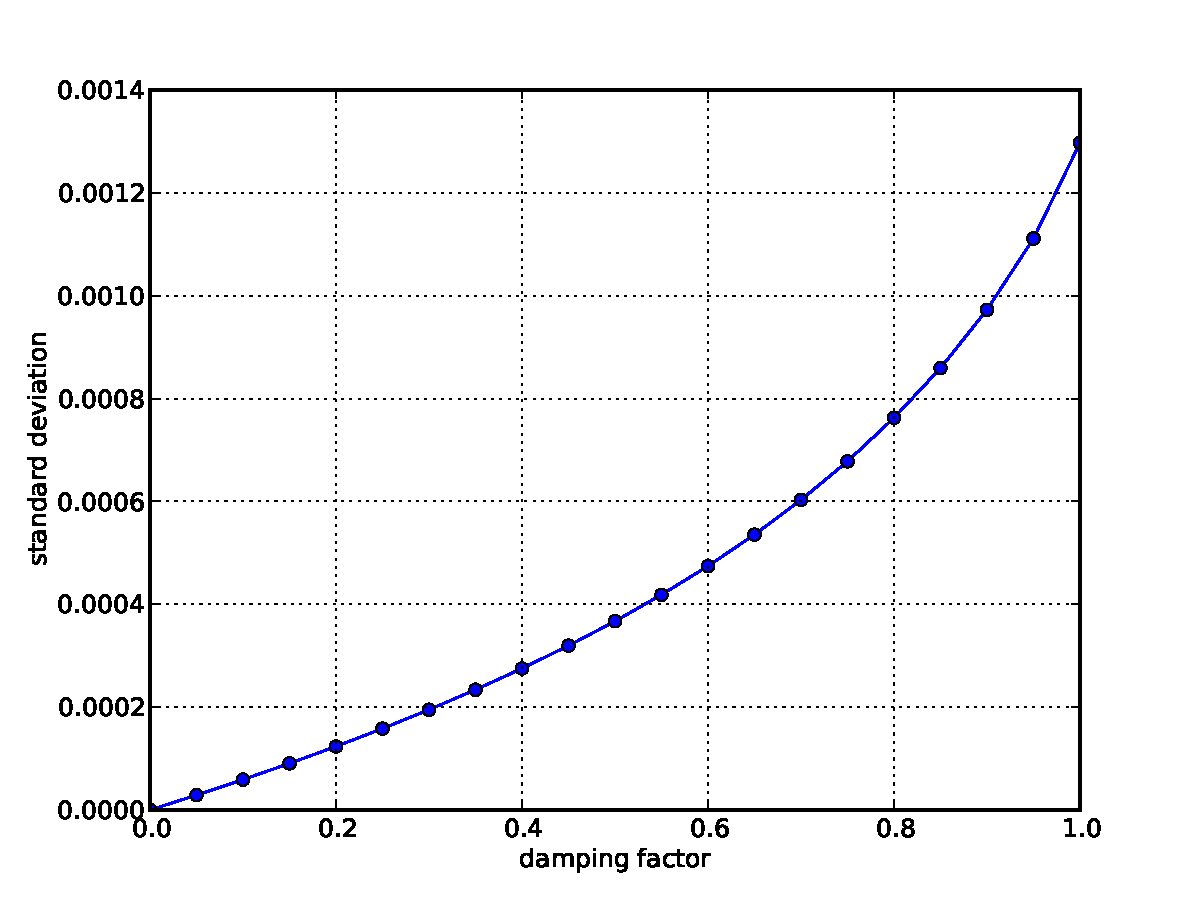
\includegraphics[width=0.75\textwidth]{standard_deviation}
 \caption{Damping value and standard deviation of PageRank scores. \label{fig:std}}

 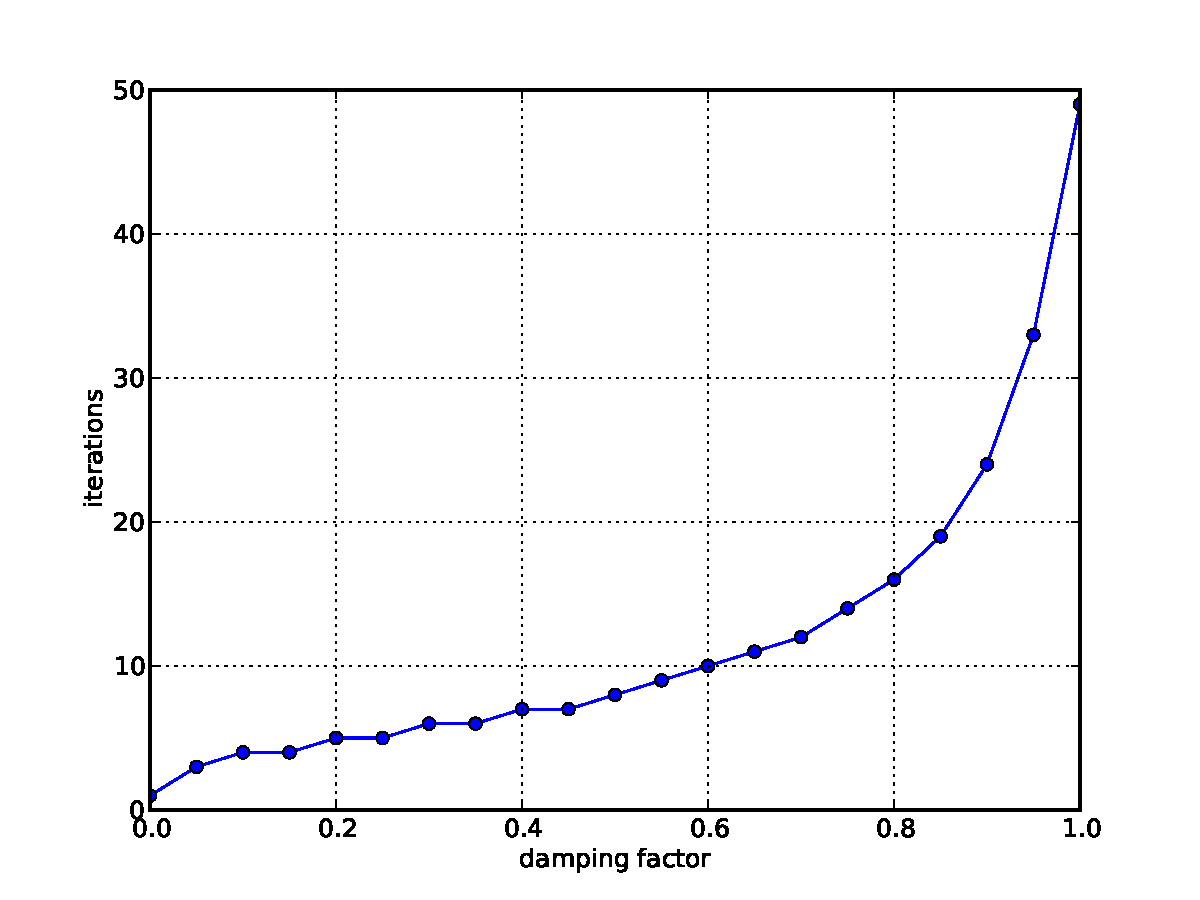
\includegraphics[width=0.75\textwidth]{iterations}
 \caption{Damping value and number of iterations required for convergence of PageRank scores ($\epsilon=\num{1e-4}$). \label{fig:iterations}}
\end{figure}

We clearly see that for small values of $\alpha$, the algorithm takes less iterations to converge and the standard deviation is smaller, compared to larger values of $\alpha$.

Assume a random surfer. With probability $\alpha$, he follows a link of the current page, with probability $1 − \alpha$ he surfs to a random page.
As $\alpha\rightarrow{}0$, the web has a link between any two pages and we have lost the original hyperlink structure of the web.
When $\alpha\rightarrow{}1$, the original hyperlink structure is taken more in account. 

Clearly, important pages (i.e., pages that happen to be linked by many other pages, or by few important ones) will be visited more often when $\alpha$ is large~\cite{ams}. However, when we take a large value of $\alpha$, the convergence of the power method will be very slow. Additionally, contrary to popular belief, $\alpha\approx1$ does not deliver ``better'' PageRank values~\cite{function}. Intuitively this is easily explained: we don't surf on the web just clicking on hyperlinks all the time. 

In conclusion, a good trade-off between meaningful PageRank values and convergence rate is achieved using the frequently used $\alpha=0.85$.


% 
% \autoref{tab:simple2} shows the distribution of the PageRank values of the pages as the number of iterations approaches infinity.
% 
% \begin{table}[hbpt]
%   \centering\footnotesize
%  \begin{tabular}{c c S S S S S}
%   \toprule
%       && \multicolumn{5}{c}{PageRank value of node} \\\cmidrule(l){3-7}
% {$i$} && \multicolumn{1}{c}{0} & \multicolumn{1}{c}{1}  & \multicolumn{1}{c}{2}  & \multicolumn{1}{c}{3}  & \multicolumn{1}{c}{4}  \\ \midrule
% 0     && 0.2000 & 0.2000 & 0.2000 & 0.2000 & 0.2000 \\
% 1     && 0.0400 & 0.1400 & 0.2067 & 0.3067 & 0.3067 \\
% 2     && 0.0613 & 0.0813 & 0.1280 & 0.3147 & 0.4147 \\
% 3     && 0.0829 & 0.1136 & 0.1407 & 0.2380 & 0.4247 \\
% 4     && 0.0849 & 0.1264 & 0.1643 & 0.2634 & 0.3609 \\
% 5     && 0.0722 & 0.1146 & 0.1568 & 0.2786 & 0.3778 \\
% \vdots&& \multicolumn{1}{c}{\vdots} & \multicolumn{1}{c}{\vdots} & \multicolumn{1}{c}{\vdots} & \multicolumn{1}{c}{\vdots} & \multicolumn{1}{c}{\vdots} \\
% % 6     && 0.0756 & 0.1117 & 0.1499 & 0.2706 & 0.3924 \\
% % 7     && 0.0785 & 0.1163 & 0.1535 & 0.2656 & 0.3862 \\
% % 8     && 0.0772 & 0.1165 & 0.1552 & 0.2695 & 0.3816 \\
% % 9     && 0.0763 & 0.1149 & 0.1538 & 0.2704 & 0.3846 \\
% 10    && 0.0769 & 0.1151 & 0.1534 & 0.2690 & 0.3856 \\
% \vdots&& \multicolumn{1}{c}{\vdots} & \multicolumn{1}{c}{\vdots} & \multicolumn{1}{c}{\vdots} & \multicolumn{1}{c}{\vdots} & \multicolumn{1}{c}{\vdots} \\
% 15    && 0.0769 & 0.1154 & 0.1539 & 0.2692 & 0.3846 \\
% %\vdots&& \multicolumn{1}{c}{\vdots & \vdots & \vdots & \vdots & \vdots \\
%   \bottomrule
%  \end{tabular}
%   \caption{Distribution of PageRank values of the nodes of the graph \emph{sample-tiny.txt} in the $i$th iteration.\label{tab:simple2}}
% \end{table}

 

% 
% \begin{figure}[hbpt] \centering
%  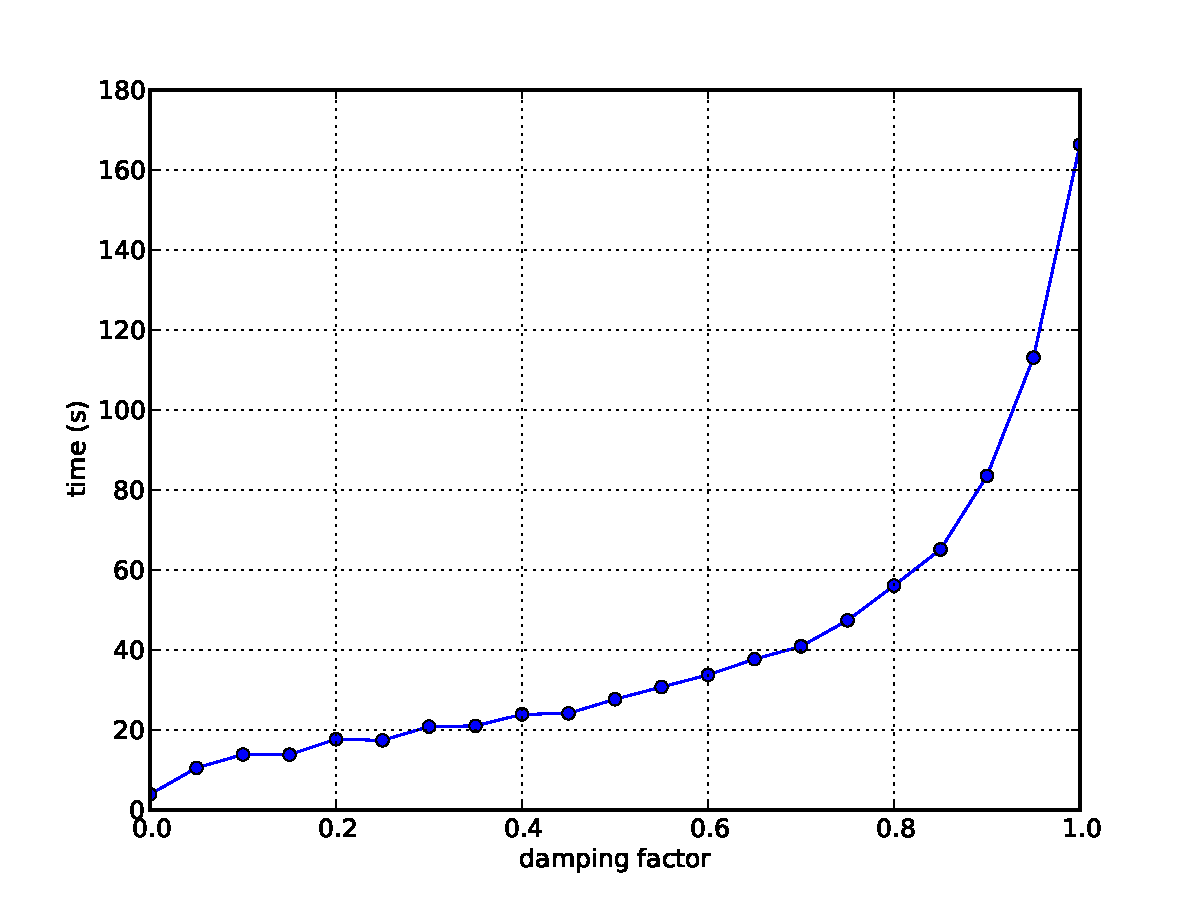
\includegraphics[width=0.75\textwidth]{times}
%  \caption{Damping value and computation time required for convergence of PageRank scores ($\epsilon=\num{1e-4}$). \label{fig:times}}
% \end{figure}

\clearpage
\section{Topical Pagerank}

Using an initial PageRank vector where the initial values are 0.02 for normal nodes, and 0.5 for the topic X nodes, after 

we get following results
pagerank of 8614504 is 0.00310119751126
pagerank of 10936880 is 0.0023332770172
pagerank of 8848271 is 0.00196661281637



\clearpage
\bibliographystyle{alpha}
\bibliography{biblio}
\nocite{*}
\end{document}
